\chapter{Plasticidad neural, aprendizaje y memoria}\label{ch:b3:learning-memory}

En 1953 un cirujano extirpó la parte interna de ambos lóbulos
temporales a un hombre joven con epilepsia intratable. Las crisis
remitieron; el paciente, conocido durante cincuenta años como H.M., no
volvió a formar ningún recuerdo duradero de un suceso. Podía mantener
una conversación, aprender a trazar una estrella en un espejo tan bien
como cualquiera ---y negar cada día haber visto la tarea--- y recordaba
su infancia. La memoria, se vio, no era una sola cosa, y la formación
de nuevos recuerdos de sucesos dependía de una estructura del tamaño de
un pulgar. Qué cambia en un encéfalo cuando aprende es la pregunta más
antigua de la neurociencia, y su respuesta, elaborada en una babosa de
mar con veinte mil neuronas y en cortes de \omterm{def:b3:learning-memory:kinds}{hipocampo} de rata, es que
las sinapsis cambian de fuerza según lo que pasa por ellas ---una regla
que Donald Hebb adivinó en 1949 y que una molécula, el \omterm{prop:b3:learning-memory:nmda}{receptor NMDA},
resultó poner en práctica. Este capítulo trata esa regla y su
maquinaria, los circuitos que la emplean para almacenar lugares y
sucesos, la matemática que dice qué puede aprender y cuánto puede
guardar un sistema así, y la señal de recompensa que le dice qué merece
la pena aprender.

\section{Clases de memoria y dónde residen}

\begin{definition}[Formas de aprendizaje y de memoria]\label{def:b3:learning-memory:kinds}
\index{habituación}\index{sensibilización}\index{condicionamiento}\index{memoria declarativa}\index{memoria procedimental}\index{consolidación}\index{hipocampo}
El aprendizaje más simple es el \emph{no asociativo}: la
\emph{habituación}, una respuesta que decae ante un estímulo inocuo
repetido, y la \emph{sensibilización}, una respuesta acrecentada tras
un estímulo nocivo. El aprendizaje \emph{asociativo} enlaza dos
sucesos: en el \emph{condicionamiento clásico} (Pávlov) un estímulo
neutro que predice una recompensa o un castigo acaba provocando la
respuesta; en el \emph{condicionamiento operante} se repite una acción
que es recompensada. La memoria humana se divide en memoria
\emph{declarativa} ---hechos y sucesos, evocados conscientemente,
dependientes del \emph{hipocampo} y del lóbulo temporal medial--- y
memoria \emph{no declarativa} ---destrezas y hábitos (cuerpo estriado,
\omterm{def:b3:nervous-systems:plan}{cerebelo}), miedo condicionado (amígdala), preactivación (corteza)---,
expresada en el desempeño sin evocación. Un recuerdo se guarda primero
en una forma lábil a corto plazo, que dura de segundos a horas, y se
\emph{consolida} a lo largo de horas o años en una forma estable a
largo plazo que ya no necesita el hipocampo y reside en la corteza.
\end{definition}

\begin{proof}[Evidencia]
Scoville y Milner (1957) describieron a H.M.: tras la extirpación de
ambos \omterm{def:b3:learning-memory:kinds}{hipocampos} y de la corteza vecina, su inteligencia y sus
recuerdos anteriores a la operación quedaron en buena medida intactos y
su memoria de trabajo era normal mientras atendiera a algo, pero no
podía formar recuerdo nuevo alguno de ningún suceso ni de ningún hecho.
Aprendía destrezas motoras a ritmo normal a lo largo de los días
mientras negaba haber practicado ---de modo que la memoria de destrezas
no necesitaba el hipocampo--- y recordaba el pasado remoto mejor que
los años inmediatamente anteriores a la cirugía, así que el \omterm{def:b3:learning-memory:kinds}{hipocampo}
hacía falta para fijar los recuerdos declarativos y, durante un tiempo,
para retenerlos, no para almacenarlos siempre. Monos y ratas con
lesiones equivalentes mostraron la misma disociación, y el estudio de
un solo paciente reorganizó todo un campo.
\end{proof}

\section{La regla de Hebb y su molécula}

\begin{definition}[Plasticidad hebbiana, LTP y LTD]\label{def:b3:learning-memory:ltp}
\index{regla de Hebb}\index{potenciación a largo plazo}\index{depresión a largo plazo}\index{plasticidad dependiente del momento de las espigas}
Hebb (1949) propuso que, cuando una neurona presináptica participa
repetidamente en hacer descargar a una postsináptica, la conexión entre
ambas se refuerza ---``las células que descargan juntas se conectan
juntas''. La \emph{potenciación a largo plazo} (LTP) es su forma
experimental: una ráfaga breve de estimulación de alta frecuencia sobre
una vía deja más fuertes las sinapsis que activó, durante horas en un
corte y durante semanas en un animal. La LTP es \emph{específica de la
entrada} (solo cambian las sinapsis estimuladas), \emph{asociativa}
(una entrada débil emparejada con una fuerte sobre la misma célula
queda potenciada) y necesita \emph{\omterm{def:b3:structural-biology:allostery}{cooperatividad}} entre entradas para
despolarizar la célula. La \emph{depresión a largo plazo} (LTD) es su
contraria, producida por una actividad prolongada de baja frecuencia.
En la \emph{plasticidad dependiente del momento de las espigas} el
signo lo fija el orden: una espiga presináptica unos milisegundos
\emph{antes} que la postsináptica refuerza la sinapsis, y una justo
\emph{después} la debilita, dentro de una ventana de unos
\qty{20}{ms} a cada lado ---de modo que una sinapsis aprende a
predecir, no solo a correlacionar.
\end{definition}

\begin{proposition}[El receptor NMDA como detector de coincidencias]\label{prop:b3:learning-memory:nmda}
\index{receptor NMDA}\index{receptor AMPA}\index{CaMKII}\index{CREB}\index{espina dendrítica}
En las sinapsis excitadoras el glutamato actúa sobre dos receptores. El
receptor \emph{AMPA} se abre al unirse el glutamato y lleva la
corriente sináptica ordinaria. El receptor \emph{NMDA} une glutamato,
pero al potencial de reposo lo bloquea un ion de magnesio alojado en su
poro; solo cuando la membrana postsináptica se despolariza ---por
muchas entradas a la vez o por un potencial de acción que
retropropaga--- se expulsa el magnesio y el canal conduce, dejando
entrar calcio. El \omterm{prop:b3:learning-memory:nmda}{receptor NMDA} se abre, por tanto, solo cuando la
liberación presináptica (glutamato) coincide con la actividad
postsináptica (despolarización): es la puerta ``y'' de Hebb en una sola
proteína. El calcio que entra en una \emph{\omterm{prop:b3:learning-memory:nmda}{espina dendrítica}} activa la
cinasa \emph{CaMKII}, que fosforila los \omterm{prop:b3:learning-memory:nmda}{receptores AMPA} y hace que
entren más en la sinapsis desde una reserva ---la sinapsis es más
fuerte en cuestión de minutos (LTP temprana). En cambio, una subida de
calcio grande y lenta activa la fosfatasa calcineurina, que retira
\omterm{prop:b3:learning-memory:nmda}{receptores AMPA}: la LTD. La potenciación que dura más de unas pocas
horas (LTP tardía) necesita proteína nueva: las cinasas alcanzan el
núcleo, el factor de transcripción \emph{CREB} enciende genes y la
espina crece y puede dividirse ---la misma exigencia de expresión
génica que separa la memoria a corto plazo de la memoria a largo plazo
en todos los animales estudiados.
\end{proposition}

\begin{proof}[Evidencia]
Bliss y L\o mo (1973) estimularon la vía perforante hacia el \omterm{def:b3:learning-memory:kinds}{hipocampo}
del conejo con un tren de pulsos y hallaron la respuesta evocada
agrandada durante horas ---la primera LTP. Collingridge (1983) mostró
que un bloqueante del \omterm{prop:b3:learning-memory:nmda}{receptor NMDA} (AP5) impedía la inducción de la
LTP, pero no la respuesta sináptica ordinaria; Morris (1986) infundió
AP5 en el \omterm{def:b3:learning-memory:kinds}{hipocampo} de ratas y comprobó que ya no podían aprender la
posición de una plataforma oculta en una piscina de agua, aunque
nadaban y veían con normalidad; y los ratones en los que el \omterm{prop:b3:learning-memory:nmda}{receptor
NMDA} se suprimió solo en la región \omterm{def:b3:learning-memory:hippocampus}{CA1} del \omterm{def:b3:learning-memory:kinds}{hipocampo} carecían tanto de
LTP allí como de memoria espacial. El mismo receptor, en el mismo
lugar, era necesario para el cambio sináptico y para el aprendizaje.
\end{proof}

\begin{omfigure}
\begin{tikzpicture}[every node/.style={font=\scriptsize}, >=stealth]
  % presynaptic terminal
  \draw[thick, omDef, fill=omDef!12] (0,2.2) .. controls (0,3.4) and (4,3.4) .. (4,2.2) -- (4,1.7) -- (0,1.7) -- cycle;
  \node at (2,2.8) {terminal presináptico};
  \foreach \p in {(0.8,2.0),(1.6,2.1),(2.6,2.0),(3.3,2.1)} \draw[thick, fill=omDef!40] \p circle (0.17);
  \foreach \p in {(1.2,1.45),(2.0,1.5),(2.9,1.42)} \fill[omProp] \p circle (0.06);
  \node[right, omProp] at (3.3,1.45) {glutamato};
  % postsynaptic spine
  \draw[thick, omMeth!70!black, fill=omMeth!10] (-0.6,1.1) -- (4.4,1.1) -- (4.4,-1.2) -- (-0.6,-1.2) -- cycle;
  \node at (0.6,-0.9) {espina dendrítica};
  % AMPA
  \draw[thick, fill=omMeth!45] (0.2,0.85) rectangle (0.6,1.35); \node[below, align=center] at (0.1,0.8) {AMPA:\\entra Na$^{+}$};
  \draw[->, thick] (0.4,1.7) -- (0.4,0.95);
  % NMDA with Mg
  \draw[thick, fill=omThm!35] (2.4,0.85) rectangle (2.9,1.35); \fill[gray!70] (2.65,1.1) circle (0.09); \node[right, font=\tiny] at (2.95,1.1) {bloqueo por Mg$^{2+}$};
  \node[below, align=center] at (2.65,0.8) {NMDA: necesita glutamato\\\emph{y} despolarización};
  \draw[->, thick, omThm] (2.65,0.15) -- (2.65,-0.5) node[below] {Ca$^{2+}$};
  % downstream
  \node[draw, rounded corners, fill=omThm!15, font=\tiny] (cam) at (5.6,0.3) {CaMKII};
  \draw[->, thick] (2.9,-0.5) -- (cam);
  \node[draw, rounded corners, fill=omMeth!25, font=\tiny, align=center] (ampa) at (8.2,1.0) {se insertan más receptores AMPA:\\LTP temprana (minutos)};
  \node[draw, rounded corners, fill=omMeth!25, font=\tiny, align=center] (creb) at (8.2,-0.5) {CREB, proteínas nuevas,\\crecimiento de la espina: LTP tardía (horas+)};
  \draw[->, thick] (cam) -- (ampa.west); \draw[->, thick] (cam) -- (creb.west);
  \node[draw, rounded corners, fill=omDef!15, font=\tiny, align=center] (ltd) at (8.2,-1.8) {Ca$^{2+}$ lento y pequeño: calcineurina,\\se retira AMPA: LTD};
  \draw[->, thick, dashed] (2.9,-0.7) .. controls (4.5,-1.6) .. (ltd.west);
\end{tikzpicture}

{\small El \omterm{prop:b3:learning-memory:nmda}{receptor NMDA} como puerta de Hebb. El glutamato por sí solo
abre los \omterm{prop:b3:learning-memory:nmda}{receptores AMPA}; el canal NMDA conduce únicamente cuando la
espina está además despolarizada y su magnesio se marcha. El calcio que
entonces entra fija el futuro de la sinapsis: una subida rápida y
grande la refuerza; una lenta y pequeña la debilita.}
\end{omfigure}

\begin{omfigure}
\begin{tikzpicture}
\begin{axis}[
  width=6.6cm, height=5.2cm,
  axis x line=bottom, axis y line=left,
  xmin=-20, xmax=120, ymin=0, ymax=220,
  xlabel={minutos}, ylabel={respuesta sináptica (\%)},
  xlabel style={font=\small, at={(axis description cs:0.5,-0.12)}, anchor=north}, ylabel style={font=\small},
  tick label style={font=\scriptsize}, xtick={0,30,60,90,120}, ytick={0,100,200},
  clip=false,
]
\addplot[only marks, mark=*, mark size=1pt, omDef] coordinates {(-18,100) (-15,98) (-12,102) (-9,99) (-6,101) (-3,100) (2,195) (5,180) (8,172) (11,168) (15,165) (20,162) (30,160) (40,158) (50,157) (60,156) (70,156) (80,155) (90,155) (100,154) (110,154) (120,154)};
\addplot[only marks, mark=o, mark size=1pt, gray] coordinates {(-18,100) (-12,101) (-6,99) (2,102) (8,100) (15,101) (30,100) (45,99) (60,101) (75,100) (90,100) (105,101) (120,100)};
\draw[->, thick, omThm] (axis cs:0,215) -- (axis cs:0,200); \node[font=\scriptsize, omThm, anchor=south] at (axis cs:0,216) {tétanos};
\node[font=\scriptsize, omDef, anchor=south west] at (axis cs:35,168) {vía estimulada: LTP};
\node[font=\scriptsize, gray, anchor=north west] at (axis cs:35,95) {vía de control: sin cambios};
\end{axis}
\begin{axis}[
  at={(7.6cm,0)}, anchor=south west,
  width=6.6cm, height=5.2cm,
  axis x line=middle, axis y line=middle,
  xmin=-60, xmax=60, ymin=-60, ymax=100,
  xlabel={$t_{\text{pre}} - t_{\text{post}}$ (ms)}, ylabel={$\Delta w$ (\%)},
  xlabel style={font=\small, at={(axis description cs:0.5,-0.06)}, anchor=north}, ylabel style={font=\small, at={(axis description cs:0.5,1.02)}, anchor=south},
  tick label style={font=\scriptsize}, xtick={-40,-20,20,40}, ytick={-40,40,80},
  clip=false,
]
\addplot[very thick, omMeth!70!black, domain=-60:-0.5, samples=60] {80*exp(x/15)};
\addplot[very thick, omThm, domain=0.5:60, samples=60] {-45*exp(-x/25)};
\node[font=\scriptsize, omMeth!70!black, anchor=south east] at (axis cs:-8,62) {pre antes que post: LTP};
\node[font=\scriptsize, omThm, anchor=north west] at (axis cs:8,-22) {post antes que pre: LTD};
\end{axis}
\end{tikzpicture}

{\small Izquierda: \omterm{def:b3:learning-memory:ltp}{potenciación a largo plazo} ---tras un tétanos breve,
la respuesta de la vía estimulada sigue agrandada durante horas
mientras que una vía no estimulada hacia las mismas células queda sin
cambios (especificidad de entrada). Derecha: la ventana temporal de las
espigas ---la sinapsis se refuerza si la espiga presináptica va delante
y se debilita si va detrás.}
\end{omfigure}

\begin{theorem}[Qué aprende una sinapsis hebbiana]\label{thm:b3:learning-memory:hebb}
\index{aprendizaje hebbiano!componente principal}\index{regla de Oja}
Sea una neurona que recibe entradas $\mathbf{x} = (x_{1},\dots,x_{n})$ a
través de pesos $\mathbf{w}$ y responde linealmente, $y = \mathbf{w}\cdot\mathbf{x}$.
La \omterm{def:b3:learning-memory:ltp}{regla de Hebb}, $\Delta\mathbf{w} = \eta\, y\,\mathbf{x}$, da, en
promedio sobre las entradas,
\[
\langle\Delta\mathbf{w}\rangle = \eta\,C\,\mathbf{w}, \qquad C =
\langle\mathbf{x}\mathbf{x}^{\mathsf{T}}\rangle ,
\]
donde $C$ es la matriz de correlación de las entradas. Los pesos crecen
sin cota, y crecen más deprisa a lo largo del autovector de $C$ con el
mayor autovalor: la sinapsis acaba detectando el patrón de entrada que
está presente más a menudo ---la \emph{componente principal} de sus
entradas. Con un término que penaliza los pesos grandes, la \emph{\omterm{thm:b3:learning-memory:hebb}{regla
de Oja}} $\Delta\mathbf{w} = \eta\, y\,(\mathbf{x} - y\,\mathbf{w})$, el
vector de pesos converge a ese autovector normalizado a longitud
unidad, y la neurona se convierte en un detector estable de la
correlación dominante en lo que ve.
\end{theorem}
\begin{proof}
Sustituyendo $y = \mathbf{w}\cdot\mathbf{x} = \mathbf{x}^{\mathsf{T}}
\mathbf{w}$ en la \omterm{def:b3:learning-memory:ltp}{regla de Hebb} resulta $\Delta\mathbf{w} = \eta\,\mathbf{x}
\mathbf{x}^{\mathsf{T}}\mathbf{w}$, cuyo promedio sobre las entradas
(con $\mathbf{w}$ cambiando despacio) es $\eta C\mathbf{w}$. $C$ es
simétrica y semidefinida positiva, de modo que tiene autovectores
ortogonales $\mathbf{e}_{k}$ con autovalores $\lambda_{k} \ge 0$;
escribiendo $\mathbf{w} = \sum_{k}
a_{k}\mathbf{e}_{k}$, cada componente cumple $\Delta a_{k} = \eta\lambda_{k}
a_{k}$ y crece como $(1 + \eta\lambda_{k})^{t}$, así que la componente
del mayor autovalor acaba dominando la dirección de $\mathbf{w}$
mientras su longitud diverge. La \omterm{thm:b3:learning-memory:hebb}{regla de Oja} promedia a $\eta(C\mathbf{w} -
(\mathbf{w}^{\mathsf{T}}C\mathbf{w})\mathbf{w})$; en un punto fijo
$C\mathbf{w} = (\mathbf{w}^{\mathsf{T}}C\mathbf{w})\mathbf{w}$, de modo
que $\mathbf{w}$ es un autovector con $\lambda = \mathbf{w}^{\mathsf{T}}
C\mathbf{w} = \lambda|\mathbf{w}|^{2}$, y por tanto $|\mathbf{w}| = 1$;
el punto fijo del mayor autovalor es el estable (una perturbación hacia
otro autovector se encoge, porque el autovalor de ese autovector es
menor), lo que aquí se admite.
\end{proof}

\begin{example}[Dos entradas]\label{ex:b3:learning-memory:two-inputs}
Una neurona recibe dos entradas que suelen estar activas a la vez, de modo que $C =
\begin{pmatrix} 1 & 0.8 \\ 0.8 & 1\end{pmatrix}$. Los autovectores son
$(1,1)/\sqrt{2}$, con autovalor $1.8$, y $(1,-1)/\sqrt{2}$, con
autovalor $0.2$. Partiendo de $\mathbf{w} = (1, 0)$, la \omterm{def:b3:learning-memory:ltp}{regla de Hebb},
tras muchos pasos pequeños, gira $\mathbf{w}$ hacia $(1,1)$: la neurona
aprende a responder a las dos entradas \emph{juntas} y a ignorar las
raras ocasiones en que solo una descarga ---ha extraído la correlación.
Con la \omterm{thm:b3:learning-memory:hebb}{regla de Oja} los pesos se asientan en $(0.71, 0.71)$. Este es el
sentido en el que las sinapsis hebbianas aprenden lo que va junto, y
por eso la propiedad asociativa de la LTP, emparejar una entrada débil
con una fuerte, se sigue de la regla.
\end{example}

\section{Una babosa que aprende}

\begin{proposition}[Sensibilización en \emph{Aplysia}]\label{prop:b3:learning-memory:aplysia}
\index{Aplysia}\index{facilitación presináptica}\index{AMPc}\index{PKA}
La babosa de mar \emph{Aplysia} retira la branquia cuando se le toca el
sifón, un reflejo de unas pocas docenas de neuronas identificables. Una
descarga en la cola la \emph{sensibiliza}: la retirada ante un roce
leve queda acrecentada, durante minutos tras una descarga y durante
semanas tras varias. Kandel y sus colaboradores (de los años setenta a
los noventa) rastrearon el cambio hasta la sinapsis entre la neurona
sensorial del sifón y la neurona motora de la branquia. La descarga en
la cola excita una \omterm{def:b3:nervous-systems:cells}{interneurona} que libera serotonina sobre el terminal
de la neurona sensorial; la serotonina eleva el AMP cíclico, que activa
la proteína cinasa A, que fosforila y cierra un canal de potasio; los
potenciales de acción del terminal se ensanchan, entra más calcio y se
libera más transmisor por espiga ---la \emph{\omterm{prop:b3:learning-memory:aplysia}{facilitación
presináptica}}, un cambio covalente que dura minutos. Las descargas
repetidas envían la cinasa al núcleo, donde activa CREB, que enciende
genes que construyen nuevos terminales sinápticos: la memoria a largo
plazo son más sinapsis, y la bloquean los inhibidores de la síntesis de
proteínas administrados durante el entrenamiento, pero no después. La
\emph{\omterm{def:b3:learning-memory:kinds}{habituación}} es lo contrario, una depresión de la misma sinapsis;
y el \emph{\omterm{def:b3:learning-memory:kinds}{condicionamiento} clásico}, emparejar el roce con la
descarga, refuerza la facilitación en las sinapsis que estaban activas
justo antes de que llegara la serotonina ---una coincidencia hebbiana
puesta en práctica presinápticamente, por una adenilato-ciclasa a la
que estimulan el calcio y la serotonina juntos.
\end{proposition}

\begin{omfigure}
\begin{tikzpicture}[every node/.style={font=\scriptsize}, >=stealth]
  \node[draw, thick, rounded corners, fill=omDef!20, minimum width=2cm] (sn) at (0,0) {neurona sensorial del sifón};
  \node[draw, thick, rounded corners, fill=omMeth!25, minimum width=2cm] (mn) at (6.2,0) {neurona motora de la branquia};
  \node[draw, thick, rounded corners, fill=omProp!30, align=center] (in) at (2.8,2.4) {interneurona facilitadora\\(serotonina)};
  \node[left] at (-2.1,0) {roce}; \draw[->, thick] (-2.0,0) -- (sn);
  \draw[->, very thick] (sn) -- (mn) node[pos=0.45, below, align=center, font=\tiny] {la sinapsis\\que cambia};
  \draw[->, thick] (mn) -- (8.4,0) node[right] {la branquia se retira};
  \node[above] at (2.8,3.1) {descarga en la cola}; \draw[->, thick] (2.8,3.05) -- (in);
  \draw[->, thick, omProp] (in) -- (2.8,0.25);
  \node[right, align=left, font=\tiny] at (6.6,1.6) {serotonina $\to$ AMPc $\to$ PKA $\to$ canal de K$^{+}$ cerrado\\$\to$ espiga más ancha, más Ca$^{2+}$, más transmisor (minutos)\\repetido: PKA $\to$ CREB $\to$ terminales nuevos (semanas)};
\end{tikzpicture}

{\small El circuito de \omterm{def:b3:learning-memory:kinds}{sensibilización} de \emph{Aplysia}. La serotonina
de una \omterm{def:b3:nervous-systems:cells}{interneurona} actúa sobre el terminal sensorial, y la misma
sinapsis lleva la memoria a corto plazo como un canal fosforilado y la
memoria a largo plazo como terminales nuevos.}
\end{omfigure}

\begin{omfigure}
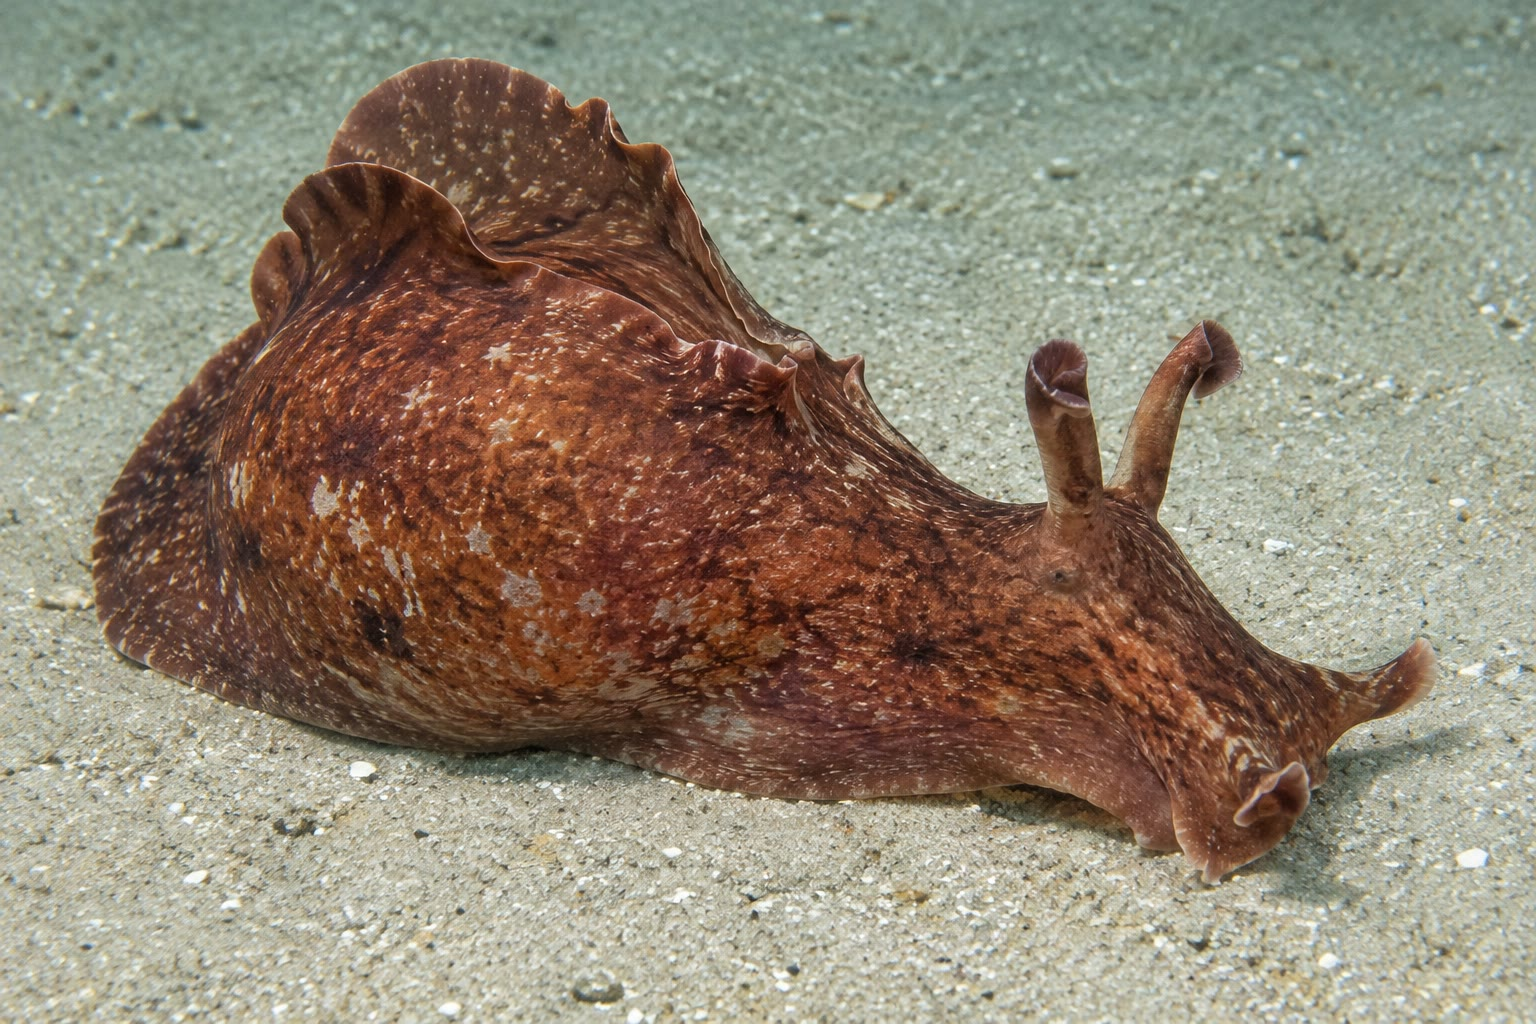
\includegraphics[width=0.46\linewidth]{images/book5/ai/b5-19-aplysia.jpg}\hspace{0.04\linewidth}
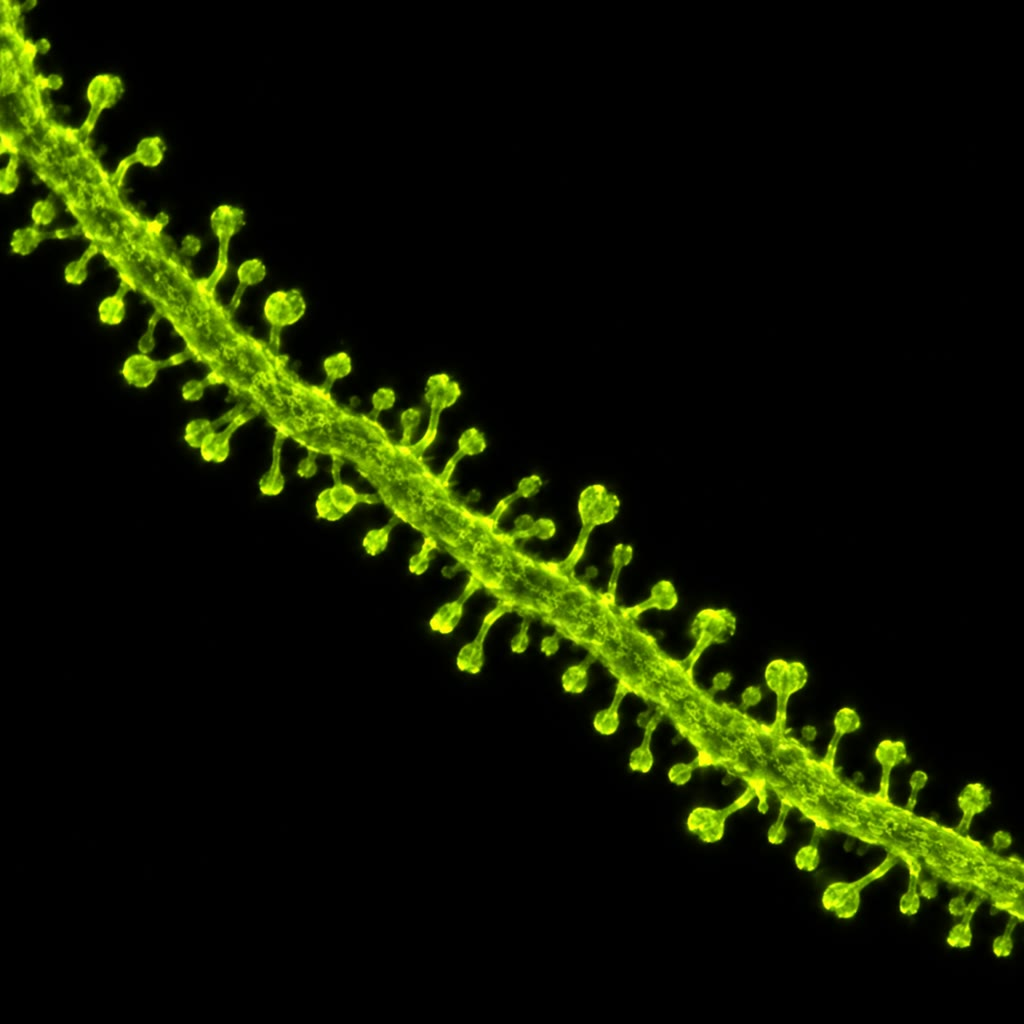
\includegraphics[width=0.36\linewidth]{images/book5/ai/b5-19-dendritic-spines.jpg}

{\small Izquierda: \emph{Aplysia californica}, cuyas neuronas, pocas y
grandes, permiten hallar y registrar la sinapsis de un recuerdo.
Derecha: una dendrita tachonada de espinas, cada una el lado
postsináptico de una sinapsis excitadora y cada una un compartimento
cuyo calcio decide su propio destino.}
\end{omfigure}

\section{Circuitos para lugares y sucesos}

\begin{definition}[El circuito hipocampal]\label{def:b3:learning-memory:hippocampus}
\index{giro dentado}\index{CA3}\index{CA1}\index{célula de lugar}\index{célula de rejilla}\index{completado de patrones}\index{reactivación}
La entrada cortical alcanza el \omterm{def:b3:learning-memory:kinds}{hipocampo} a través de la corteza
entorrinal y atraviesa tres etapas: el \emph{giro dentado}, cuyas
células granulares superan en número a sus entradas y descargan de
forma escasa (lo que separa patrones parecidos); \emph{CA3}, cuyas
células piramidales se conectan de forma recurrente entre sí y reciben
cada una miles de sinapsis de las demás ---una red
\emph{autoasociativa} capaz de completar un patrón almacenado a partir
de un fragmento---; y \emph{CA1}, que compara la salida de CA3 con la
entrada directa y devuelve el resultado a la corteza. En una rata que
explora un recinto, una célula piramidal del \omterm{def:b3:learning-memory:kinds}{hipocampo} descarga solo
cuando el animal está en un lugar ---una \emph{célula de lugar}
(O'Keefe, 1971)--- y unos cientos de ellas cartografían el recinto; en
la corteza entorrinal, aguas arriba, las \emph{células de rejilla}
(Moser, 2005) descargan en los vértices de una retícula hexagonal que
cubre el espacio, un sistema de coordenadas a partir del cual se
construyen los campos de lugar. Durante el sueño y el reposo, las
secuencias de células de lugar que descargaron durante un recorrido se
\emph{reactivan} a gran velocidad, y bloquear esa reactivación
deteriora el recuerdo del recorrido: el \omterm{def:b3:learning-memory:kinds}{hipocampo} le ensaya a la
corteza los caminos del día.
\end{definition}

\begin{omfigure}
\begin{tikzpicture}[every node/.style={font=\scriptsize}, >=stealth]
  % trisynaptic loop
  \node[draw, thick, rounded corners, fill=gray!15, align=center] (ec) at (0,0) {corteza entorrinal\\(células de rejilla)};
  \node[draw, thick, rounded corners, fill=omDef!20, align=center] (dg) at (3.2,1.4) {giro dentado:\\separación de patrones};
  \node[draw, thick, rounded corners, fill=omProp!30, align=center] (ca3) at (7.2,1.4) {CA3, recurrente:\\completado de patrones};
  \node[draw, thick, rounded corners, fill=omMeth!25, align=center] (ca1) at (7.2,-1.4) {CA1:\\compara y emite};
  \draw[->, thick] (ec) -- (dg); \draw[->, thick] (dg) -- (ca3); \draw[->, thick] (ca3) -- (ca1); \draw[->, thick] (ca1) -- (ec) node[pos=0.3, below, sloped, font=\tiny] {de vuelta a la corteza};
  \draw[->, thick, dashed] (ec) -- (ca1.north west) node[pos=0.7, above, sloped, font=\tiny] {vía directa};
  \draw[->, thick, omProp!80!black] (ca3.north) .. controls (6.6,2.6) and (7.8,2.6) .. (ca3.north east) node[pos=0.5, above, font=\tiny] {colaterales recurrentes};
  % place field map
  \begin{scope}[xshift=10.4cm, yshift=-0.2cm]
    \draw[thick] (0,0) rectangle (3,2.4); \node[below] at (1.5,-0.05) {recinto, visto desde arriba};
    \foreach \p/\c in {(0.7,1.8)/omThm, (2.1,1.9)/omDef, (1.4,0.9)/omMeth, (2.5,0.6)/omProp} { \fill[\c!60] \p circle (0.32); \fill[\c!90] \p circle (0.16); }
    \node[above] at (1.5,2.45) {campos de descarga de cuatro células de lugar};
  \end{scope}
\end{tikzpicture}

{\small Izquierda: el bucle hipocampal ---separación en el \omterm{def:b3:learning-memory:hippocampus}{giro
dentado}, almacenamiento y completado en el \omterm{def:b3:learning-memory:hippocampus}{CA3} recurrente, comparación
en \omterm{def:b3:learning-memory:hippocampus}{CA1}. Derecha: cada \omterm{def:b3:learning-memory:hippocampus}{célula de lugar} descarga en una región del
recinto; entre todas cartografían el espacio.}
\end{omfigure}

\begin{proposition}[Cuánto guarda una red autoasociativa]\label{prop:b3:learning-memory:capacity}
\index{red de Hopfield}\index{capacidad de memoria}
Una red de $N$ neuronas, conectada cada una con todas las demás
mediante pesos hebbianos $w_{ij} \propto \sum_{\mu}\xi_{i}^{\mu}\xi_{j}^{\mu}$
sumados sobre los patrones binarios almacenados $\xi^{\mu}$, recupera
un patrón almacenado a partir de una pista corrupta o parcial
asentándose en él como atractor (Hopfield, 1982). Lo hace de manera
fiable para hasta unos $P
\approx 0.14N$ patrones aleatorios; más allá, los patrones interfieren
y la recuperación se derrumba. El \omterm{def:b3:learning-memory:hippocampus}{CA3} de una rata, con unas
$3\times 10^{5}$ células piramidales, podría según esta estimación
guardar unos $4\times 10^{4}$ patrones ---el orden de los lugares o
episodios distintos que un animal encuentra en una estación--- y su
descarga escasa (un pequeño porcentaje de células activas en cada
patrón) eleva aún más la capacidad. El \omterm{def:b3:learning-memory:hippocampus}{completado de patrones} a partir
de una pista es lo que permite que un olor o una esquina evoquen una
escena entera; el precio es que los recuerdos parecidos se funden, cosa
a la que se resiste la separación del \omterm{def:b3:learning-memory:hippocampus}{giro dentado}.
\end{proposition}
\admitted

\begin{method}[Poner a prueba la memoria y su mecanismo]\label{met:b3:learning-memory:tests}
\index{laberinto acuático de Morris}\index{condicionamiento del miedo}\index{engrama}
(1) Una tarea espacial: el \omterm{met:b3:learning-memory:tests}{laberinto acuático de Morris} ---una rata
nada en agua opaca hasta una plataforma oculta en un lugar fijo,
aprende su posición a partir de las claves de la sala a lo largo de
varios días, y se la evalúa por el tiempo que pasa buscando en el
cuadrante correcto cuando se retira la plataforma; las lesiones
hipocampales, los bloqueantes de NMDA y la pérdida de la LTP abolen
cada uno el aprendizaje. (2) Una tarea asociativa: el \omterm{met:b3:learning-memory:tests}{condicionamiento
del miedo} ---un tono emparejado con una descarga en la pata acaba
provocando inmovilización; el recuerdo depende de la amígdala, y una
versión específica del contexto, del \omterm{def:b3:learning-memory:kinds}{hipocampo}. (3) Una prueba de
mecanismo: bloquéese el candidato (un fármaco, una \omterm{def:b3:genetic-engineering:transgenic}{supresión génica}
restringida a una región y a un momento) y muéstrese que el aprendizaje
falla mientras la percepción y el movimiento no. (4) El engrama:
márquense las neuronas activas durante el aprendizaje con un canal
sensible a la luz (\cref{ch:b3:nervous-systems}) y reactívense después
con luz ---el animal se inmoviliza en un contexto seguro, como si
recordara; silenciarlas bloquea la evocación. La memoria está en
células identificables y en sus sinapsis, y puede encenderse y
apagarse.
\end{method}

\begin{omfigure}
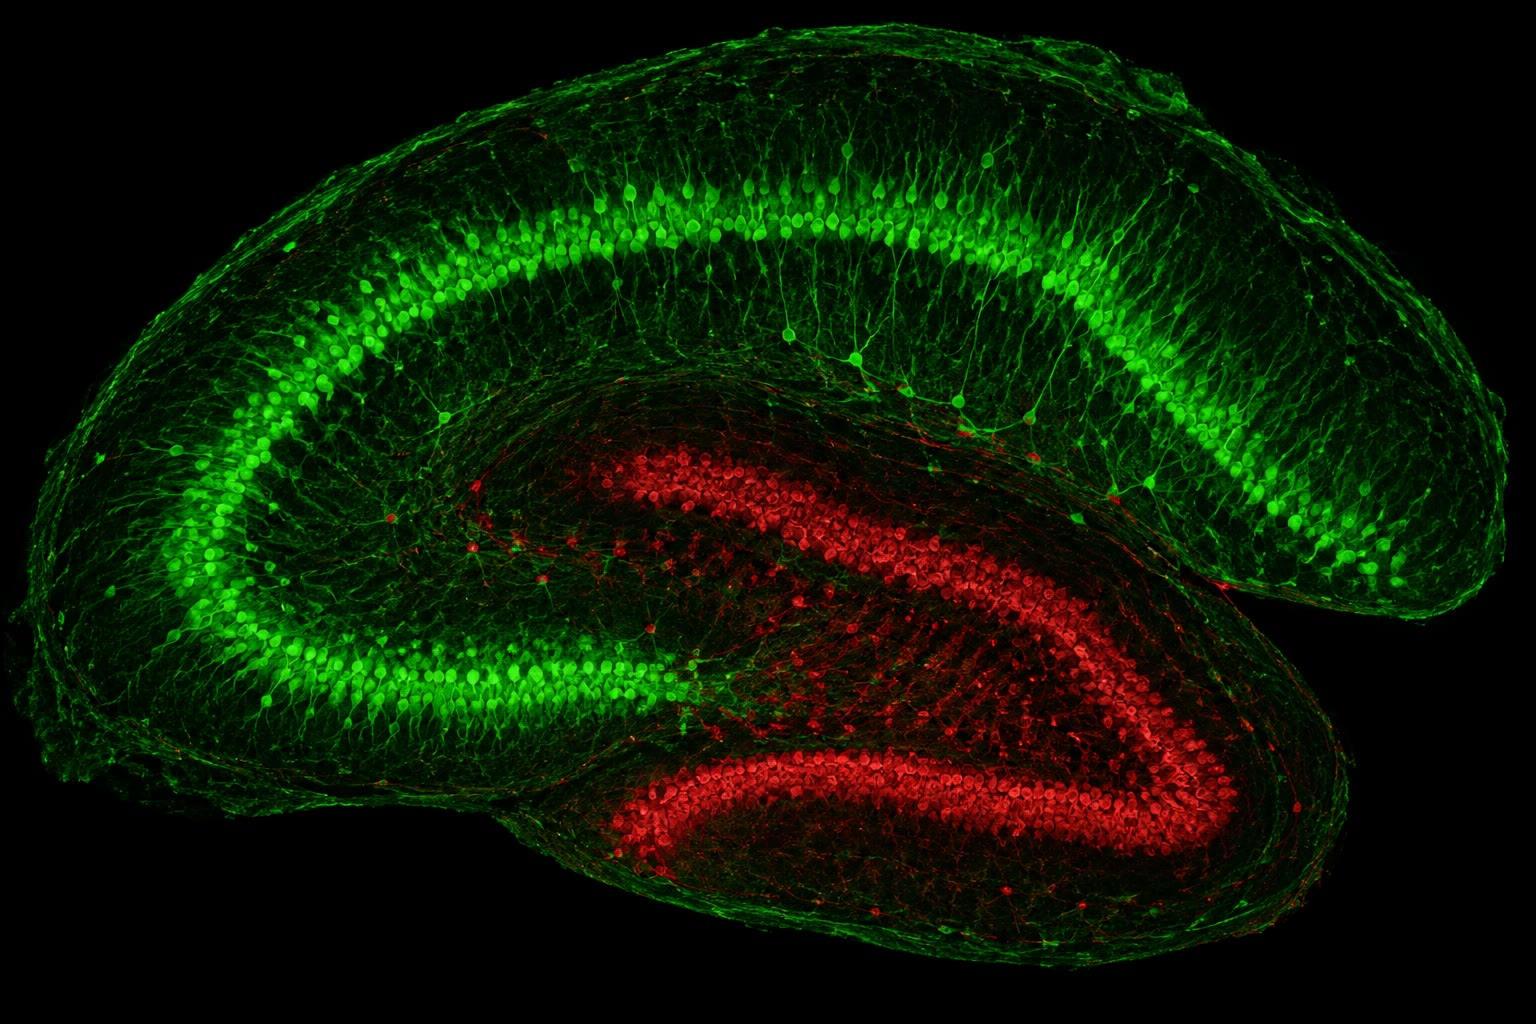
\includegraphics[width=0.56\linewidth]{images/book5/ai/b5-19-hippocampus-section.jpg}

{\small Un corte del \omterm{def:b3:learning-memory:kinds}{hipocampo} de un roedor: la banda curva de células
piramidales (verde) desde \omterm{def:b3:learning-memory:hippocampus}{CA3} hasta \omterm{def:b3:learning-memory:hippocampus}{CA1} y el \omterm{def:b3:learning-memory:hippocampus}{giro dentado} (rojo)
engarzado en ella. Todo recuerdo espacial del animal pasa por este
bucle.}
\end{omfigure}

\section{Recompensa, predicción y la plasticidad de toda una vida}

\begin{proposition}[Aprender por error de predicción]\label{prop:b3:learning-memory:rescorla}
\index{regla de Rescorla--Wagner}\index{error de predicción}\index{dopamina}
Sea $V$ el valor que un animal atribuye a una clave y $\lambda$ la
recompensa que la sigue. La \omterm{prop:b3:learning-memory:rescorla}{regla de Rescorla--Wagner} (1972) dice que
en cada ensayo el valor cambia en una fracción $\alpha$ del
\emph{\omterm{prop:b3:learning-memory:rescorla}{error de predicción}}:
\[
\Delta V = \alpha\,(\lambda - V), \qquad
V_{n} = \lambda\bigl(1 - (1-\alpha)^{n}\bigr) ,
\]
de modo que el aprendizaje es rápido al principio y se frena a medida
que la predicción mejora, se detiene cuando la recompensa está
totalmente predicha y se invierte (extinción) cuando la recompensa se
retira. Cuando se presentan dos claves juntas comparten una sola
predicción, de modo que una clave que no añade nada a una predicción ya
hecha no se aprende (\emph{bloqueo}). Schultz (1997) registró las
neuronas dopaminérgicas del mesencéfalo en monos y halló que descargan
ante una recompensa inesperada, callan ante una totalmente predicha y
caen por debajo de su nivel basal cuando una recompensa predicha no
llega: difunden $\lambda - V$, el propio \omterm{prop:b3:learning-memory:rescorla}{error de predicción}, al cuerpo
estriado y a la corteza, donde la dopamina abre el paso a la
plasticidad en las sinapsis que estuvieron activas hace poco. Aprender
qué predice una recompensa es plasticidad hebbiana con un tercer factor
que dice si el resultado fue mejor o peor de lo esperado ---y las
drogas de abuso, al impulsar directamente la dopamina, falsifican un
``mejor de lo esperado'' permanente.
\end{proposition}
\begin{proof}
La recursión $V_{n+1} = V_{n} + \alpha(\lambda - V_{n})$ da
$\lambda - V_{n+1} = (1-\alpha)(\lambda - V_{n})$, de modo que el error
se encoge geométricamente, $\lambda - V_{n} = (1-\alpha)^{n}\lambda$
desde $V_{0} =
0$, de donde sale la fórmula. Para dos claves $A$ y $B$ presentadas
juntas la predicción es $V_{A} + V_{B}$; si $A$ se entrenó primero
hasta $V_{A} = \lambda$, el error en los ensayos compuestos es cero y
$B$ no adquiere nada.
\end{proof}

\begin{omfigure}
\begin{tikzpicture}
\begin{axis}[
  width=6.6cm, height=5.0cm,
  axis x line=bottom, axis y line=left,
  xmin=0, xmax=25, ymin=0, ymax=1.1,
  xlabel={ensayo $n$}, ylabel={$V_{n}/\lambda$},
  xlabel style={font=\small, at={(axis description cs:0.5,-0.14)}, anchor=north}, ylabel style={font=\small},
  tick label style={font=\scriptsize}, xtick={0,5,10,15,20,25}, ytick={0,0.5,1},
  clip=false,
]
\addplot[very thick, omDef, domain=0:12, samples=13] {1-0.8^x};
\addplot[very thick, omDef, domain=12:25, samples=14] {(1-0.8^12)*0.8^(x-12)};
\draw[dashed, gray] (axis cs:12,0) -- (axis cs:12,1.05);
\node[font=\scriptsize, anchor=north west, align=left] at (axis cs:0.5,0.98) {recompensa dada:\\adquisición};
\node[font=\scriptsize, anchor=north west, align=left] at (axis cs:14,0.98) {recompensa retirada:\\extinción};
\end{axis}
\begin{axis}[
  at={(7.6cm,0)}, anchor=south west,
  width=6.6cm, height=5.0cm,
  ybar, bar width=14pt,
  axis x line=bottom, axis y line=left,
  ymin=-1.2, ymax=1.5,
  symbolic x coords={recompensa inesperada, recompensa predicha, recompensa omitida},
  xtick=data, ytick={-1,0,1}, yticklabels={caída,basal,ráfaga},
  ylabel={descarga dopaminérgica},
  x tick label style={font=\scriptsize, align=center, text width=1.9cm}, ylabel style={font=\small}, tick label style={font=\scriptsize},
  clip=false,
]
\addplot[fill=omThm!50, draw=omThm] coordinates {(recompensa inesperada,1.2) (recompensa predicha,0.05) (recompensa omitida,-1.0)};
\end{axis}
\end{tikzpicture}

{\small Izquierda: la curva de aprendizaje de Rescorla--Wagner con
$\alpha = 0.2$ ---aproximación geométrica al valor de la recompensa y
luego extinción cuando la recompensa cesa. Derecha: las neuronas
dopaminérgicas informan del \omterm{prop:b3:learning-memory:rescorla}{error de predicción} ---una ráfaga ante una
sorpresa, nada ante una recompensa predicha, una caída cuando falta una
recompensa predicha.}
\end{omfigure}

\begin{definition}[Períodos críticos y las enfermedades de la plasticidad]\label{def:b3:learning-memory:critical}
\index{período crítico}\index{dominancia ocular}\index{adicción}\index{enfermedad de Alzheimer}
La plasticidad es máxima en ventanas del desarrollo. Hubel y Wiesel (en
los años sesenta) taparon un ojo a un gatito durante unas semanas
después del nacimiento: la corteza visual, gobernada normalmente por
ambos ojos en columnas alternantes, pasó a estar gobernada casi por
completo por el ojo abierto, y el ojo privado quedó funcionalmente
ciego de por vida ---mientras que la misma privación en un gato adulto
no cambiaba nada. Esos \emph{períodos críticos}, para la visión, para
el lenguaje, para el canto de las aves, se cierran cuando maduran los
circuitos inhibidores y la matriz extracelular se endurece, y pueden
reabrirse un poco con fármacos y entrenamiento. Las patologías de la
plasticidad lo son de dosis y de diana: la \emph{adicción} es
aprendizaje impulsado por un \omterm{prop:b3:learning-memory:rescorla}{error de predicción} falsificado, que
construye hábitos que sobreviven al placer; el estrés postraumático es
un recuerdo de miedo sobreconsolidado por las hormonas del estrés; y la
\emph{enfermedad de Alzheimer} empieza donde empieza la \omterm{def:b3:learning-memory:kinds}{memoria
declarativa}, en la corteza entorrinal y el \omterm{def:b3:learning-memory:kinds}{hipocampo}, con la pérdida de
sinapsis ---que acompaña a la demencia mejor que cualquier recuento de
placas--- antes de la pérdida de neuronas.
\end{definition}

\begin{remark}[De qué está hecha la memoria]\label{rem:b3:learning-memory:what}
Un recuerdo no es una grabación, sino un cambio en las fuerzas y en el
número de las sinapsis, repartido por las células que estaban activas
cuando se formó, fijado por una regla que refuerza lo que descarga
junto, regulado por una señal que dice si el resultado importaba, y
ensayado durante el sueño hasta que la corteza lo sostiene por su
cuenta. La regla es la de Hebb, la puerta es el \omterm{prop:b3:learning-memory:nmda}{receptor NMDA}, la señal
es la dopamina, el ensayo es la \omterm{def:b3:learning-memory:hippocampus}{reactivación}, y la matemática dice qué
puede guardar un sistema así y por qué confunde lo parecido. Todo
experimento que ha encendido o apagado un recuerdo ---con un
bloqueante, con un gen, con luz--- lo ha hallado en esas sinapsis, en
esas células. H.M. murió en 2008; su encéfalo, cortado y fotografiado,
mostró la lesión que había enseñado a todo un campo, y nada más.
\end{remark}

\section{Ejercicios}

\begin{exercise}[$\star$]\label{exo:b3:learning-memory:1}
Distíngase la \omterm{def:b3:learning-memory:kinds}{memoria declarativa} de la no declarativa a partir del
desempeño de H.M., y nómbrese una región encefálica para cada una de
cuatro clases de memoria no declarativa.
\end{exercise}

\begin{exercise}[$\star$]\label{exo:b3:learning-memory:2}
Enúnciese el postulado de Hebb y las tres propiedades de la LTP que se
siguen de él.
\end{exercise}

\begin{exercise}[$\star$]\label{exo:b3:learning-memory:3}
Explíquese por qué el \omterm{prop:b3:learning-memory:nmda}{receptor NMDA} es un detector de coincidencias y
qué le ocurre a la LTP cuando su bloqueante AP5 se aplica antes del
tétanos y cuando se aplica después.
\end{exercise}

\begin{exercise}[$\star$]\label{exo:b3:learning-memory:4}
En \emph{Aplysia}, ¿qué distingue la \omterm{def:b3:learning-memory:kinds}{sensibilización} a corto plazo de
la \omterm{def:b3:learning-memory:kinds}{sensibilización} a largo plazo en el plano molecular, y qué
experimento lo muestra?
\end{exercise}

\begin{exercise}[$\star\star$]\label{exo:b3:learning-memory:5}
Con $\alpha = 0.3$, ¿cuántos ensayos hacen falta hasta que $V$ alcanza
el \qty{90}{\%} de $\lambda$? Si la recompensa se retira entonces,
¿cuántos ensayos hasta que $V$ cae por debajo del \qty{10}{\%}? ¿Por
qué son simétricas la adquisición y la extinción en este modelo, y lo
son en los animales?
\end{exercise}

\begin{exercise}[$\star\star$]\label{exo:b3:learning-memory:6}
Dos entradas tienen $C = \begin{pmatrix}1 & 0.5\\ 0.5 & 1\end{pmatrix}$.
Hállense los autovectores y los autovalores, y dígase hacia qué
dirección gira los pesos la \omterm{def:b3:learning-memory:ltp}{regla de Hebb} y qué detecta entonces la
neurona. Aplíquese un paso de la \omterm{thm:b3:learning-memory:hebb}{regla de Oja} desde $\mathbf{w} = (1,0)$ con la entrada $\mathbf{x}
= (1,1)$ y $\eta = 0.1$.
\end{exercise}

\begin{exercise}[$\star\star$]\label{exo:b3:learning-memory:7}
Una espina tiene un volumen de \qty{0.1}{fL}. La entrada de $500$ iones
de calcio, ¿en cuánto eleva su concentración libre (en
$\unit{\micro mol/L}$) si los tampones fijan de inmediato el
\qty{95}{\%}? Compárese con los \qty{0.1}{\micro mol/L} de reposo y con
la $K_{d}$ de la calmodulina, activadora de CaMKII, de alrededor de
\qty{1}{\micro mol/L}.
\end{exercise}

\begin{exercise}[$\star\star$]\label{exo:b3:learning-memory:8}
Explíquese el bloqueo con la \omterm{prop:b3:learning-memory:rescorla}{regla de Rescorla--Wagner} y dese el
registro dopaminérgico que corresponde a cada etapa.
\end{exercise}

\begin{exercise}[$\star\star$]\label{exo:b3:learning-memory:9}
Predíganse los resultados de (a) la supresión del \omterm{prop:b3:learning-memory:nmda}{receptor NMDA}
restringida a \omterm{def:b3:learning-memory:hippocampus}{CA1}, (b) un inhibidor de la síntesis de proteínas
administrado durante el entrenamiento, (c) el mismo inhibidor
administrado un día después, (d) la \omterm{def:b3:learning-memory:hippocampus}{reactivación} optogenética, en un
contexto nuevo, de las células del \omterm{def:b3:learning-memory:hippocampus}{giro dentado} que estuvieron activas
durante un \omterm{met:b3:learning-memory:tests}{condicionamiento del miedo}.
\end{exercise}

\begin{exercise}[$\star\star\star$]\label{exo:b3:learning-memory:10}
Muéstrese que bajo la sola \omterm{def:b3:learning-memory:ltp}{regla de Hebb} la longitud de $\mathbf{w}$
crece sin cota, y que la \omterm{thm:b3:learning-memory:hebb}{regla de Oja} tiene $|\mathbf{w}| = 1$ en todo
punto fijo. ¿Por qué es un problema biológico el crecimiento sin cota,
y qué mecanismos (escalado sináptico, LTD, sueño) podrían corresponder
al término normalizador?
\end{exercise}

\begin{exercise}[$\star\star\star$]\label{exo:b3:learning-memory:11}
El \omterm{def:b3:learning-memory:hippocampus}{CA3} de una rata tiene $3\times 10^{5}$ células; el de un ser humano,
unos $2\times 10^{6}$. Estímese la capacidad de Hopfield de cada uno.
¿Por qué es la estimación una mala medida de cuántos recuerdos guarda
una persona, y qué añade al cuadro el papel del \omterm{def:b3:learning-memory:kinds}{hipocampo} en la
\omterm{def:b3:learning-memory:kinds}{consolidación}?
\end{exercise}

\begin{exercise}[$\star\star\star$]\label{exo:b3:learning-memory:12}
Los gatitos privados de la visión de un ojo durante semanas pierden el
territorio cortical de ese ojo; los adultos no. Explíquese mediante la
competencia hebbiana por qué gana el ojo abierto, por qué la privación
binocular tiene menos efecto que la monocular y qué cierra el \omterm{def:b3:learning-memory:critical}{período
crítico}.
\end{exercise}

\section{Problema: una sinapsis que recuerda}

\begin{problem}[{Problema de fin de semana --- un recuerdo seguido
desde el calcio de una espina hasta una rata en un laberinto: la
aritmética del calcio en la inducción, una neurona hebbiana que
converge en lo que sus entradas comparten, una curva de aprendizaje
marcada por el error de predicción y la capacidad de un hipocampo, para
terminar en la concentración de calcio que induce la LTP, los ensayos
que necesita una rata y los patrones que su CA3 puede guardar}]
\label{pb:b3:learning-memory:1}
Datos: una espina de volumen \qty{0.08}{fL}; cada canal NMDA lleva
$10^{3}$ Ca$^{2+}$ por apertura de \qty{50}{ms}; una sinapsis tiene
$10$ \omterm{prop:b3:learning-memory:nmda}{receptores NMDA}; se tampona el \qty{98}{\%} del calcio que entra;
calcio libre de reposo, \qty{0.1}{\micro mol/L}; CaMKII se activa por
encima de \qty{2}{\micro mol/L} de calcio libre, y la calcineurina
entre $0.3$ y \qty{1}{\micro mol/L}. Hebb: dos entradas con $C = \begin{pmatrix}1 &
0.6\\ 0.6 & 1\end{pmatrix}$, $\eta = 0.1$. Rescorla--Wagner: $\alpha =
0.15$. Capacidad: \omterm{def:b3:learning-memory:hippocampus}{CA3} de rata, $3\times 10^{5}$ células, $P = 0.14N$;
una rata explora $20$ lugares nuevos al día.

\medskip
\noindent\textbf{Parte I --- El calcio.}
\begin{enumerate}
  \item Los diez \omterm{prop:b3:learning-memory:nmda}{receptores NMDA} se abren una vez. ¿Cuántos iones de
        calcio entran, cuántos quedan libres y qué subida de
        concentración supone eso en la espina?
  \item ¿Se activa CaMKII? ¿Y si solo se abren dos receptores
        (glutamato liberado, pero la espina apenas despolarizada)?
  \item Con dos receptores abiertos, ¿qué enzima queda dentro de su
        intervalo y qué le ocurre a la sinapsis? Explíquese cómo un
        solo ion puede producir tanto LTP como LTD.
  \item El calcio se bombea al exterior con una constante de tiempo de
        \qty{20}{ms}. ¿Por qué deben llegar las entradas en decenas de
        milisegundos para sumar su calcio, y cómo fija esto la ventana
        temporal de las espigas?
  \item Una espina dista \qty{0.5}{\micro m} de su vecina en la
        dendrita. Explíquese por qué el tamponamiento y el cuello
        estrecho de la espina mantienen la señal de calcio dentro de
        una sola espina, y por qué eso importa para la especificidad de
        entrada.
  \item El bloqueo por magnesio se levanta hacia los \qty{-30}{mV}. Una
        sola sinapsis AMPA despolariza la espina \qty{5}{mV} desde
        \qty{-70}{mV}. ¿Cuántas entradas sincrónicas (o qué otra cosa)
        hacen falta para desbloquear los \omterm{prop:b3:learning-memory:nmda}{receptores NMDA}? ¿Qué dice
        esto sobre la \omterm{def:b3:structural-biology:allostery}{cooperatividad}?
\end{enumerate}

\medskip
\noindent\textbf{Parte II --- Una neurona hebbiana.}
\begin{enumerate}[resume]
  \item Hállense los autovalores y los autovectores de $C$.
  \item Partiendo de $\mathbf{w} = (1, 0)$, aplíquese la \omterm{def:b3:learning-memory:ltp}{regla de Hebb}
        promediada $\mathbf{w} \leftarrow \mathbf{w} + \eta C\mathbf{w}$
        durante tres pasos. ¿Qué ángulo forma $\mathbf{w}$ con la
        dirección $(1,1)$ tras cada uno?
  \item Tras muchos pasos, ¿cuál es la razón $w_{2}/w_{1}$ y qué le
        ocurre a $|\mathbf{w}|$?
  \item Aplíquese un paso de la \omterm{thm:b3:learning-memory:hebb}{regla de Oja} promediada $\mathbf{w} \leftarrow \mathbf{w} +
        \eta\,(C\mathbf{w} - (\mathbf{w}^{\mathsf{T}}C\mathbf{w})
        \mathbf{w})$ desde $(0.8, 0.8)$. ¿Hacia dónde se mueve?
  \item La neurona responde ahora a las dos entradas juntas. Si
        descarga solo la entrada 2 (cosa rara), ¿cuánto vale $y$
        respecto del caso conjunto, con $\mathbf{w} = (0.71, 0.71)$?
  \item Explíquese en una frase cómo la asociatividad de la LTP (una
        entrada débil emparejada con una fuerte se refuerza) es este
        teorema en acción.
\end{enumerate}

\medskip
\noindent\textbf{Parte III --- La curva de aprendizaje.}
\begin{enumerate}[resume]
  \item Con $\alpha = 0.15$, calcúlese $V_{n}/\lambda$ tras $5$, $10$ y
        $20$ ensayos.
  \item ¿Cuántos ensayos hacen falta para alcanzar el \qty{95}{\%} de
        $\lambda$?
  \item Una rata aprende un laberinto en aproximadamente ese número de
        ensayos. Si se duplica la recompensa, ¿predice el modelo un
        aprendizaje más rápido en número de ensayos? ¿Qué cambia?
  \item La clave A se entrena hasta la asíntota, y luego se presentan A
        y B juntas con la misma recompensa durante $20$ ensayos.
        ¿Cuánto vale $V_{B}$? ¿Qué hacen las neuronas dopaminérgicas en
        los ensayos compuestos?
  \item La recompensa pasa a seguir a B sola. Descríbanse el \omterm{prop:b3:learning-memory:rescorla}{error de
        predicción} y la respuesta dopaminérgica del primer ensayo, y el
        curso de $V_{B}$.
  \item Un fármaco eleva la dopamina con independencia del resultado.
        Con la regla, explíquese por qué las acciones que preceden al
        fármaco se aprenden como si hubieran sido recompensadas,
        cualesquiera que sean sus consecuencias.
\end{enumerate}

\medskip
\noindent\textbf{Parte IV --- El \omterm{def:b3:learning-memory:kinds}{hipocampo}.}
\begin{enumerate}[resume]
  \item Capacidad de Hopfield del \omterm{def:b3:learning-memory:hippocampus}{CA3} de la rata.
  \item A $20$ lugares nuevos al día, ¿cuánto se tarda en alcanzar la
        capacidad? ¿Qué debe ocurrir para que el animal siga
        aprendiendo?
  \item La \omterm{def:b3:learning-memory:kinds}{consolidación} transfiere los recuerdos a la corteza a lo
        largo de semanas. Explíquese por qué una transferencia lenta
        protege los recuerdos corticales antiguos (interferencia
        catastrófica) y por qué el \omterm{def:b3:learning-memory:kinds}{hipocampo} es un almacén temporal.
  \item Si el \qty{3}{\%} de las células de \omterm{def:b3:learning-memory:hippocampus}{CA3} está activo en cada
        patrón, ¿cuántas células codifican un lugar y cuántos patrones
        podrían distinguirse si se exigiera que compartieran menos de
        la mitad de sus células? (Arguméntese cualitativamente por qué
        la codificación escasa eleva la capacidad.)
  \item La \omterm{def:b3:learning-memory:hippocampus}{reactivación} durante el sueño comprime un recorrido de
        \qty{10}{s} en \qty{0.5}{s}. Si la ventana temporal de las
        espigas es de \qty{20}{ms}, ¿qué separación entre las descargas
        de las \omterm{def:b3:learning-memory:hippocampus}{células de lugar} durante el recorrido se vuelve hebbiana
        en la \omterm{def:b3:learning-memory:hippocampus}{reactivación}? ¿Por qué podría ser este el sentido de la
        compresión?
  \item El recuerdo del laberinto sobrevive a una lesión hipocampal
        practicada un mes después del entrenamiento, pero no a una
        practicada un día después. Interprétese, con el patrón de
        pérdida de H.M.
  \item Resúmase: la concentración de calcio libre tras diez aperturas
        de NMDA (pregunta~1), los ensayos hasta un aprendizaje del
        \qty{95}{\%} (pregunta~14) y la capacidad del \omterm{def:b3:learning-memory:hippocampus}{CA3} de la rata
        (pregunta~19).
\end{enumerate}
\end{problem}
